% !TEX TS-program = XeLaTeX
% use the following command:
% all document files must be coded in UTF-8
\documentclass[portuguese]{textolivre}
% build HTML with: make4ht -e build.lua -c textolivre.cfg -x -u article "fn-in,svg,pic-align"

\journalname{Texto Livre}
\thevolume{16}
%\thenumber{1} % old template
\theyear{2023}
\receiveddate{\DTMdisplaydate{2022}{10}{28}{-1}} % YYYY MM DD
\accepteddate{\DTMdisplaydate{2023}{1}{5}{-1}}
\publisheddate{\DTMdisplaydate{2023}{2}{27}{-1}}
\corrauthor{Thiago Dantas}
\articledoi{10.1590/1983-3652.2023.41598}
%\articleid{NNNN} % if the article ID is not the last 5 numbers of its DOI, provide it using \articleid{} commmand 
% list of available sesscions in the journal: articles, dossier, reports, essays, reviews, interviews, editorial
\articlesessionname{articles}
\runningauthor{Dantas et al.} 
%\editorname{Leonardo Araújo} % old template
\sectioneditorname{Daniervelin Pereira}
\layouteditorname{Leonado Araújo}

\title{Máscaras pandêmicas: uma revisão sistemática sobre os impactos da máscara no reconhecimento das emoções}
\othertitle{Pandemic masks: a review systematics on the impacts of the mask on recognition of emotions}
% if there is a third language title, add here:
%\othertitle{Artikelvorlage zur Einreichung beim Texto Livre Journal}

\author[1]{Thiago Dantas~\orcid{0000-0002-9530-8707}\thanks{Email: \href{mailto:thiagodantas474@gmail.com}{thiagodantas474@gmail.com}}}
\author[1]{Julian Tejada~\orcid{0000-0003-0275-3578}\thanks{Email: \href{mailto:julian.tejada@gmail.com}{julian.tejada@gmail.com}}}
\author[2]{Raquel Meister Ko. Freitag~\orcid{0000-0002-4972-4320}\thanks{Email: \href{mailto:rkofreitag@academico.ufs.br}{rkofreitag@academico.ufs.br}}}
\affil[1]{Universidade Federal de Sergipe, Departamento de Psicologia, São Cristóvão, Sergipe, Brasil.}
\affil[2]{Universidade Federal de Sergipe, Departamento de Letras Vernáculas, São Cristóvão, Sergipe, Brasil.}

\addbibresource{Bibliografia.bib}
% use biber instead of bibtex
% $ biber article

% used to create dummy text for the template file
\definecolor{dark-gray}{gray}{0.35} % color used to display dummy texts
\usepackage{lipsum}
\SetLipsumParListSurrounders{\colorlet{oldcolor}{.}\color{dark-gray}}{\color{oldcolor}}

% used here only to provide the XeLaTeX and BibTeX logos
\usepackage{hologo}

% if you use multirows in a table, include the multirow package
\usepackage{multirow}

% provides sidewaysfigure environment
\usepackage{rotating}

% CUSTOM EPIGRAPH - BEGIN 
%%% https://tex.stackexchange.com/questions/193178/specific-epigraph-style
\usepackage{epigraph}
\renewcommand\textflush{flushright}
\makeatletter
\newlength\epitextskip
\pretocmd{\@epitext}{\em}{}{}
\apptocmd{\@epitext}{\em}{}{}
\patchcmd{\epigraph}{\@epitext{#1}\\}{\@epitext{#1}\\[\epitextskip]}{}{}
\makeatother
\setlength\epigraphrule{0pt}
\setlength\epitextskip{0.5ex}
\setlength\epigraphwidth{.7\textwidth}
% CUSTOM EPIGRAPH - END

% LANGUAGE - BEGIN
% ARABIC
% for languages that use special fonts, you must provide the typeface that will be used
% \setotherlanguage{arabic}
% \newfontfamily\arabicfont[Script=Arabic]{Amiri}
% \newfontfamily\arabicfontsf[Script=Arabic]{Amiri}
% \newfontfamily\arabicfonttt[Script=Arabic]{Amiri}
%
% in the article, to add arabic text use: \textlang{arabic}{ ... }
%
% RUSSIAN
% for russian text we also need to define fonts with support for Cyrillic script
% \usepackage{fontspec}
% \setotherlanguage{russian}
% \newfontfamily\cyrillicfont{Times New Roman}
% \newfontfamily\cyrillicfontsf{Times New Roman}[Script=Cyrillic]
% \newfontfamily\cyrillicfonttt{Times New Roman}[Script=Cyrillic]
%
% in the text use \begin{russian} ... \end{russian}
% LANGUAGE - END

% EMOJIS - BEGIN
% to use emoticons in your manuscript
% https://stackoverflow.com/questions/190145/how-to-insert-emoticons-in-latex/57076064
% using font Symbola, which has full support
% the font may be downloaded at:
% https://dn-works.com/ufas/
% add to preamble:
% \newfontfamily\Symbola{Symbola}
% in the text use:
% {\Symbola }
% EMOJIS - END

% LABEL REFERENCE TO DESCRIPTIVE LIST - BEGIN
% reference itens in a descriptive list using their labels instead of numbers
% insert the code below in the preambule:
%\makeatletter
%\let\orgdescriptionlabel\descriptionlabel
%\renewcommand*{\descriptionlabel}[1]{%
%  \let\orglabel\label
%  \let\label\@gobble
%  \phantomsection
%  \edef\@currentlabel{#1\unskip}%
%  \let\label\orglabel
%  \orgdescriptionlabel{#1}%
%}
%\makeatother
%
% in your document, use as illustraded here:
%\begin{description}
%  \item[first\label{itm1}] this is only an example;
%  % ...  add more items
%\end{description}
% LABEL REFERENCE TO DESCRIPTIVE LIST - END


% add line numbers for submission
%\usepackage{lineno}
%\linenumbers

\usepackage{calc}
\usepackage{tikz}
\usetikzlibrary{shapes.geometric}
\usetikzlibrary{arrows.meta,arrows}
\usepackage{longtable}

% enabling hyphenation on \texttt
% https://tex.stackexchange.com/questions/44361/how-to-automatically-hyphenate-within-texttt
\DeclareFontFamily{\encodingdefault}{\ttdefault}{\hyphenchar\font=`\-}

\begin{document}
\maketitle 

\begin{polyabstract}
\begin{abstract}
O uso de máscaras pandêmicas é uma das principais mudanças comportamentais trazidas pela pandemia de COVID-19, o que possivelmente tem prejudicado o Reconhecimento de Expressões Faciais (REF). Esta revisão sistemática tem como objetivo reunir e comparar metodologias e resultados de experimentos, publicados entre 2019 e 2022, que avaliam o impacto das máscaras pandêmicas no REF. Para tanto, este estudo baseou-se e dividiu-se nas recomendações do PRISMA, em três etapas: identificação, triagem e elegibilidade. A primeira etapa foi dedicada à escolha dos descritores, do recorte temporal e à aplicação destes nas bases de dados escolhidas. Na segunda etapa, foi feita a leitura dos títulos, resumos e palavras-chave, de modo a selecionar artigos que estejam de acordo com os critérios de inclusão. Os artigos selecionados nesta etapa foram colocados na plataforma Connected Papers, com a finalidade de explorar referências não identificadas via bases de dados. Na última fase, foi realizada a leitura integral e a síntese dos estudos. Finalmente, foram eleitos 11 artigos cujos resultados mostraram que as máscaras pandêmicas prejudicam o REF de modo heterogêneo. Expressões como felicidade e nojo, que dependem da região da boca para serem discriminadas, são prejudicadas. A tristeza também é prejudicada pelas máscaras pandêmicas, confundindo-se frequentemente com rostos neutros e vice-versa. Para que as descobertas sejam mais generalizáveis, os próximos estudos precisam adotar tarefas padronizadas com todas as expressões básicas e incluir expressões não básicas, como vergonha. Além disso, são recomendados a implementação de estímulos dinâmicos com variação étnica e o controle acerca do tempo de exposição.

\keywords{Máscaras \sep Emoções \sep Reconhecimento \sep Experimento}
\end{abstract}

\begin{english}
\begin{abstract}
The use of pandemic masks is one of the main behavioral changes brought about by the COVID-19 pandemic, which has possibly hampered the Facial Emotion Recognition (FER). This systematic review aims to gather and compare methodologies and results of experiments, published between 2019 and 2022, that assess the impact of pandemic masks on FER. Therefore, this study has been based and divided on the PRISMA recommendations, in three stages: identification, screening, and eligibility. The first step was dedicated to the choice of descriptors, the time frame and their application in the chosen databases. In the second step, titles, abstracts, and keywords were read to select articles that meet the inclusion criteria. The articles selected at this stage were placed on the Connected Papers platform, in order to explore unidentified references via databases. In the last phase, the full reading and the synthesis of the studies were carried out. Finally, 11 articles have been elected, whose results showed that pandemic masks harm the FER in a heterogeneous way. Expressions such as happiness and disgust, which depend on the region of the mouth to be discriminated, are harmed. Sadness is also undermined by pandemic masks, often getting confused with neutral faces and vice versa. For the findings to be more generalizable, future studies need to adopt standardized tasks with all basic expressions and include non-basic expressions such as shame. In addition, the implementation of dynamic stimuli with ethnic variation and control over exposure time are recommended.

\keywords{Mask \sep Emotion \sep Recognition \sep Experiment}
\end{abstract}
\end{english}
% if there is another abstract, insert it here using the same scheme
\end{polyabstract}

\section{Introdução}\label{sec-intro}

No dia 11 de março de 2020, a Organização Mundial da Saúde declarou que o mundo enfrentava uma pandemia causada por uma síndrome respiratória chamada Coronavirus Disease 2019 (COVID-19). A partir de então, juntamente com os demais países, o Brasil adotou o uso obrigatório de máscaras pandêmicas, que se tornaram uma das principais medidas de proteção para controlar o contágio da doença \cite{brasil_lei_2020}. Levando em conta o início da pandemia, a medida do uso obrigatório de máscaras pandêmicas\footnote{As máscaras pandêmicas são coberturas faciais da metade inferior do rosto, que podem ser de
algodão (tecido caseiro), poliéster (como a cirúrgica e a N95) ou de material filtrante especial (PFF2).} foi a estratégia mais duradoura até o momento, haja vista que, até março de 2022, era medida obrigatória em todos os estados do Brasil, tanto em ambientes fechados quanto em abertos. Em dezembro de 2021, a medida de isolamento social sofreu um afrouxamento ao mesmo tempo em que a variação Ômicron – 10 vezes mais contagiosa – se espalhava pelos países \cite{chen_extremely_2022}, momento em que a estratégia de vacinação havia alcançado quase 80\% da população brasileira com a primeira dose. Em maio de 2022 (momento em que este estudo está sendo descrito), as máscaras pandêmicas continuam sendo obrigatórias por determinação federal apenas em aeroportos, mas estados e municípios podem, por decreto, determinar a obrigatoriedade da proteção, a partir dos seus boletins técnicos sobre a taxa de infecção \cite{brasil_anvisa_2022}. Mesmo com a liberação das máscaras pandêmicas em locais fechados, instituições públicas também podem determinar seu uso à entrada de pessoas, como é o caso das universidades federais do país, que têm solicitado o uso da máscara pandêmica e o passaporte vacinal das pessoas que fazem uso de seu espaço \cite{capital_usp_2022}.  


Diante da instabilidade trazida pela COVID-19, torna-se evidente que a máscara pandêmica continuará a fazer parte do cotidiano como uma das principais medidas físicas para controlar o contágio \cite{ferguson_report_2020}. Mas, ao mesmo tempo em que é essencial, a máscara pandêmica oculta a parte inferior do rosto e, por consequência, pode prejudicar o Reconhecimento de Expressões Faciais (REF), que são fundamentais para a interação social e comunicação. 

\subsection{Emoções básicas e expressões faciais }\label{sec-conduta}

O estudo das emoções e de suas expressões é antigo, e teve como grande propulsor o naturalista inglês \citefirstlastauthor{darwin_expression_1872} \citeyear{darwin_expression_1872}, que, a partir de fotografias, mostrou que seres humanos e animais demonstram suas emoções a partir de expressões faciais. Na sua perspectiva, considerada evolucionista, as emoções são programas de ação selecionadas para o organismo lidar com situações recorrentes durante a história filogenética de sua espécie \cite{matsumoto_facial_2008, tooby_evolutionary_2008}. Cada programa de ação pressupõe que há sinais que indicam a presença de uma estrutura de eventos e condições que ocorreram durante a evolução de uma determinada emoção. Assim, circuitos neurais associados ao ‘nojo’ em seres humanos presumem um mundo em que os cheiros podres sinalizam toxinas e contaminação, por exemplo \cite{ matsumoto_facial_2008, matsumoto_facial_2008}. Internamente, a reação de ‘nojo’ é o que motiva e prepara o indivíduo para se afastar do estímulo, enquanto externamente o afastamento é acompanhado por uma reação automática e involuntária que articula os músculos do rosto de uma maneira específica: a expressão facial de ‘nojo’. Quando nos referimos a humanos, a emoção é, portanto, a experiência completa, que envolve aspectos fisiológicos e subjetivos, enquanto a expressão facial é uma mudança pública, involuntária e automática na articulação dos músculos do rosto decorrente da ativação de um programa de ação \cite{ekman_argument_1989}. 

Até a década de 1970, os sucessores de Darwin já haviam identificado pelo menos seis emoções e expressões supostamente básicas, que haviam aparecido invariavelmente nas culturas estudadas: felicidade, tristeza, medo, raiva, nojo e surpresa \cite{vasconcellos_psicopatia_2014}. Mas a pesquisa em outras culturas, muito diferentes da ocidental no aspecto linguístico, aparecia como o principal obstáculo metodológico. Com o objetivo de testar a universalidade das emoções e suas expressões, o psicólogo Paul Ekman dedicou-se à investigação em uma ilha em Papua Nova Guiné, com nativos que ainda não haviam tido contato com a cultura ocidental. Como o grande empecilho dos outros estudiosos se dava pela dificuldade de nomear as emoções, Ekman dedicou-se primeiro a assistir a vídeos de pessoas dessa cultura e a catalogar expressões faciais de seus membros. Em seguida, elaborou histórias baseadas na cultura local, com desfechos em diferentes emoções e, por último, pediu para que os participantes escolhessem a expressão emocional catalogada correspondente àquela apresentada pelo personagem na história. Com isso, Ekman confirmou que os seres humanos experimentam seis emoções básicas e cada uma possui um modo particular de expressão por meio do rosto \cite{ekman_argument_1989}. 


Na perspectiva de Ekman, denominada Abordagem da Expressão Emocional \cite{sousa_emocoes_2010}, as expressões faciais estão associadas, cada uma, a um conjunto específico de ativação de músculos do rosto, como a redução ou expansão das sobrancelhas, abertura da boca, a posição do septo nasal, a formação de cantos na boca, enquanto o seu Reconhecimento de Expressão Facial (REF) é um processo de interpretação desses sinais \cite{du_compound_2014, smith_transmitting_2005, tejada_building_2022}. A partir disso, \textcite{ekman_facial_2002} desenvolveu o Facial Action Coding System (FACS), uma taxonomia de discriminação anatômica que abrange todos os músculos faciais observáveis e maximiza o REF. Nesse sistema, cada conjunto de músculos envolvido nos movimentos faciais que compõem uma expressão é conhecido como Unidades de Ação (AU). Localmente, as AUs da área da boca parecem ser essenciais para o diagnóstico de felicidade e nojo, enquanto as AUs da região dos olhos parecem ser diagnósticas para as expressões de tristeza, medo e raiva \cite{donato_classifying_1999, du_compound_2014, tejada_building_2022}. Existem 44 AUs que são definidas pelos músculos que são ativados, sua contração e seu relaxamento. Por exemplo, a AU 4 é aquela que define a contração de dois músculos presentes nas sobrancelhas e é costumeiramente expressada por tristeza, raiva e medo \cite{donato_classifying_1999, ekman_facial_2002, ekman_pictures_1976}. O grau em que cada músculo é ativado também tem uma escala de A (leve) a E (contração máxima), e pode diferenciar tanto uma emoção quanto o nível de sua intensidade. 


\subsection{Expressões faciais e máscaras pandêmicas}\label{sec-fmt-manuscrito}

Ao considerar que cada área do rosto é responsável pela transmissão de uma informação que se relaciona à interpretação de uma emoção, é de se supor que o reconhecimento de cada expressão pode ser afetado diferentemente pela máscara pandêmica. Como destacado anteriormente, a expressão facial de felicidade aparece fortemente relacionada à área da boca, mas alguns estudos mostram que o impacto da cobertura sobre essa área do rosto pode não ser tão importante \cite{calvo_facial_2008,calvo_facial_2014}. Tais resultados dão suporte para uma vertente da literatura sobre REF que considera que as expressões são interpretadas a partir da visualização do todo, isto é, holisticamente \cite{freud_covid-19_2020, kovacs_face_2017}. Enquanto outros, na esteira do que defende Ekman como, por exemplo \textcite{wegrzyn_mapping_2017}, são categóricos ao mostrar a partir do FACS que as expressões faciais dependem de pontos críticos (neste caso, as AUs) para serem reconhecidas com precisão. Há ainda outros estudos que mostram que somente a visualização total ou parcial de um rosto não é o único aspecto que influencia no reconhecimento bem-sucedido de uma expressão facial, mas aspectos contextuais do rosto e do observador, tais como cultura \cite{kret_recognition_2018}, idade e sexo \cite{cortez_o_2021} também podem determinar o REF. 


Ao considerar as divergências teóricas e metodológicas, o presente estudo pretende verificar, a partir de uma revisão sistemática da literatura, se as máscaras diminuem o reconhecimento de expressões faciais e se esse efeito é uniforme no reconhecimento das expressões faciais. Com isso, pretende-se avaliar o papel das áreas da boca e dos olhos nesse exercício. Por fim, esta revisão tem como propósito o mapeamento das características metodológicas em termos de configuração das tarefas e de estímulos usados em experimentos. A síntese dos resultados e das metodologias empregadas por esses estudos pode destacar lacunas e ao mesmo tempo direções para pesquisas futuras.



\section{Método}\label{sec-modelo}

Esta revisão sistemática foi desenvolvida a partir das recomendações PRISMA (Preferred Reporting Items for Systematic Reviews and Meta-Analyses), apresentada por \textcite{galvao_revisao_2019}. Os termos definidos foram: \texttt{facial AND mask AND emotion AND recognition}. Buscou-se estudos descritos no formato de artigo que incluíssem esses termos no título, resumo e palavras-chave. As pesquisas foram feitas duas vezes por dois pesquisadores independentes nas bases de dados Web of Science e SCOPUS, usando o acesso CAFe do Portal de Periódicos da CAPES. O recorte temporal levou em conta o início dos primeiros casos de COVID-19 até outubro de 2021, sendo selecionados artigos com datas entre 2019, 2020, 2021 e 2022 que tivessem sido publicados até outubro de 2021. O \textit{string} usado em SCOPUS foi: \texttt{TITLE-ABS-KEY (Facial AND mask AND emotion AND recognition) AND  (LIMIT-TO (PUBYEAR,  2022)  OR  LIMIT-TO (PUBYEAR, 2021)  OR  LIMIT-TO (PUBYEAR, 2020)  OR  LIMIT-TO (PUBYEAR, 2019))  AND  (LIMIT-TO (DOCTYPE, "ar"))}. E o \textit{string} usado em Web of Sciene foi: \texttt{Facial AND mask AND emotion AND recognition (All Fields) AND 2019 OR 2020 OR 2021 OR 2022 (Publication Years) AND Article (Document Types)}. Os critérios de inclusão foram: 
\begin{enumerate*}[label=\emph{\alph*})] 
  \item apresentar metodologia experimental quantitativa;
  \item ser um trabalho que a avalie o impacto da cobertura facial (seja a condição de máscara pandêmica, apagamento de informações faciais, seja na condição de lenço) sobre o reconhecimento de expressões faciais;
  \item ter como variável dependente o desempenho no reconhecimento de expressões emocionais.
\end{enumerate*}
%a) apresentar metodologia experimental quantitativa; 
%b) ser um trabalho que a avalie o impacto da cobertura facial (seja a condição de máscara pandêmica, apagamento de informações faciais, seja na condição de lenço) sobre o reconhecimento de expressões faciais; 
%c) ter como variável dependente o desempenho no reconhecimento de expressões emocionais. 
Por outro lado, foram critérios de exclusão: 
\begin{enumerate*}[label=\emph{\alph*})] 
  \item estudos não localizados pela ferramenta Biblioshiny; 
  \item estudos que avaliem o reconhecimento de expressões faciais em máquinas, como computadores e \textit{smartphones}; 
  \item estudos com tarefas não digitais, realizadas presencialmente com fotografias. 
\end{enumerate*}
%a) estudos não localizados pela ferramenta Biblioshiny; 
%b) estudos que avaliem o reconhecimento de expressões faciais em máquinas, como computadores e \textit{smartphones}; 
%c) estudos com tarefas não digitais, realizadas presencialmente com fotografias. 
Não foram excluídos estudos de amostra não aleatória, e a ausência de grupo controle também não foi critério para exclusão.


O processo de seleção foi dividido em três etapas: identificação, triagem e elegibilidade. Na fase de identificação, a partir da aplicação dos filtros nas bases de dados, foram encontradas 95 referências (SCOPUS=36; Web of Science=44; Connected Papers=15). Na fase de triagem, os resumos advindos das bases de dados foram analisados, e 18 artigos atenderam aos critérios de inclusão. Em seguida, cada um desses trabalhos foi anexado à ferramenta Connected Papers, que oferece a possibilidade de observar conexões entre o artigo anexado e outros artigos conforme uma métrica de semelhança entre suas citações e referências. Mediante a leitura dos resumos de estudos mais similares encontrados com essa ferramenta, foram adicionados 15 artigos. Assim, ao todo, na etapa de elegibilidade, foram submetidos à leitura integral 33 artigos, dos quais 22 foram excluídos com base nos critérios de exclusão. Por fim, esta síntese qualitativa analisa e compara dados de 11 artigos (ver \Cref{fig-img-a}). Vale salientar que a ferramenta Connected Papers permitiu a seleção de três artigos não identificados nas bases de dados \cite{marini_impact_2021, noyes_effect_2021, ruba_childrens_2020}

\begin{figure}
\centering
\begin{minipage}{.85\textwidth}
 {\scriptsize
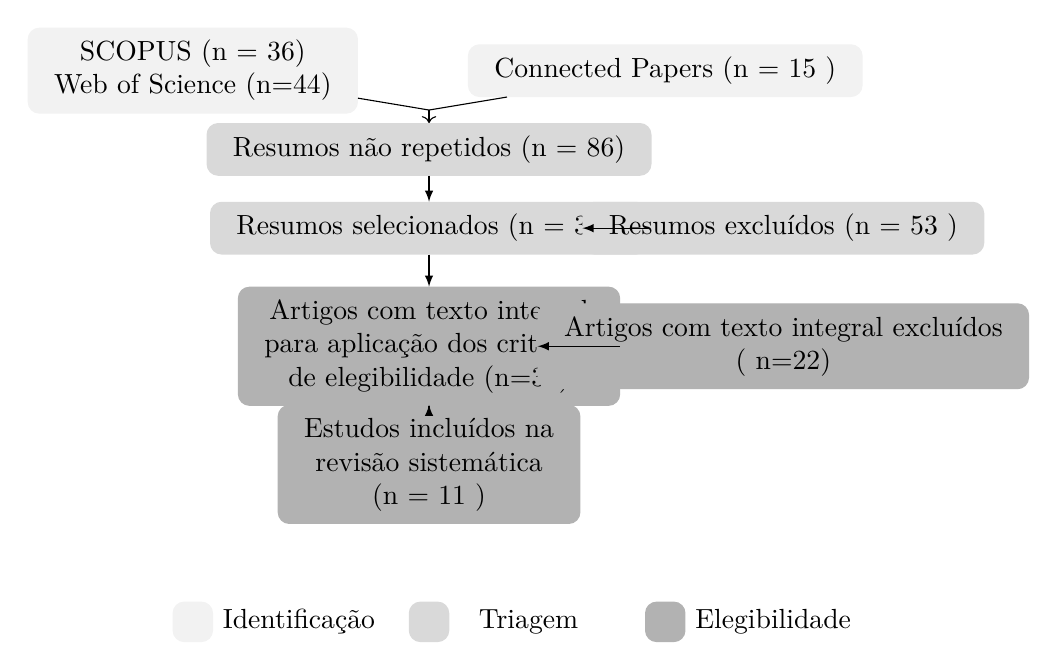
\begin{tikzpicture}[
every node/.style = {draw=black, rounded corners, fill=gray!30, 
                     minimum width=2cm, minimum height=0.5cm,
                     align=center},
every path/.style = {draw, -latex}]


\node[gray!10] (Primero)  at (0,0) {{\color{black}\begin{tabular}{c} SCOPUS (n = 36) \\ Web of Science (n=44) \end{tabular}}};
\node[gray!10] (Segundo) at (6,0) {{\color{black}\begin{tabular}{c} Connected Papers (n = 15 ) \end{tabular}}};

\node[gray!30] (Tercero) at (3,-1) {{\color{black}\begin{tabular}{c} Resumos não repetidos (n = 86) \end{tabular}}};

  \draw[-] (3,-0.5) -- (Primero);
  \draw[-] (3,-0.5) -- (Segundo);
  \draw[->] (3,-0.5) -- (Tercero);

\node[gray!30] (Quarto) at (3,-2) {{\color{black}\begin{tabular}{c}Resumos selecionados (n = 33  ) \end{tabular}}};  
\node[gray!30] (Quinto) at (7.5,-2) {{\color{black}\begin{tabular}{c}Resumos excluídos (n = 53  ) \end{tabular}}}; 
\draw   (Tercero) edge  (Quarto);
\draw   (Quarto) edge  (Quinto);

\node[gray!60] (Sexto) at (3,-3.5) {{\color{black}\begin{tabular}{c}Artigos com texto integral \\ para aplicação dos critérios \\ de elegibilidade (n=33)\end{tabular}}}; 
\node[gray!60] (Septimo) at (7.5,-3.5) {{\color{black}\begin{tabular}{c}Artigos com texto integral excluídos\\( n=22)\end{tabular}}};
\draw   (Quarto) edge  (Sexto);
\draw   (Sexto) edge  (Septimo);

\node[gray!60] (Octavo) at (3,-5) {{\color{black}\begin{tabular}{c}Estudos incluídos na \\ revisão sistemática \\ (n = 11  ) \end{tabular}}};
\draw   (Sexto) edge  (Octavo);

\draw node[gray!10, minimum size= 0.5cm] at (0,-7) [label=right:Identificação] {A};
\draw node[gray!30, minimum size= 0.5cm] at (3,-7) [label=right:Triagem] {B};
\draw node[gray!60, minimum size= 0.5cm] at (6,-7) [label=right:Elegibilidade] {E};

  
\end{tikzpicture} 
  }
\caption{Diagrama de Sistematização da Revisão.}
\label{fig-img-a}
\source{Elaboração Própria}
\end{minipage}
\end{figure}


\section{Resultados e discussão}\label{sec-organizacao}

Primeiramente, quanto à modalidade de participação, por conta da pandemia, todas as pesquisas ocorreram de modo remoto ($n=11$) (ver \Cref{tbl-01}). Como modo de cobrir expressões faciais, máscaras pandêmicas foram predominantes ($n=10$). A maioria dos estudos desenvolveu suas próprias tarefas assistidas por computador com bancos de imagens acessados pela internet, e apenas um fez uso de uma tarefa padronizada \cite{bani_behind_2021}. Quase metade ($n=7$) dos rostos dos artigos desta síntese foram retirados do banco de imagens MPI FACES \cite{ebner_facesdatabase_2010}. Dentro dos estudos que usaram máscaras pandêmicas, somente um estudo não adicionou esse estímulo via \textit{software} de edição, utilizando assim estímulos autênticos \cite{noyes_effect_2021}. Relatos acerca do tempo de exibição de cada imagem com rosto com expressão facial apareceram apenas em quatro artigos: \textcite{marini_impact_2021} e \textcite{noyes_effect_2021} limitaram todas as exibições a 1 segundo, enquanto os trabalhos de \textcite{bani_behind_2021} e \textcite{grundmann_face_2020} limitaram todas as exibições a 2 segundos. Observa-se, portanto, que o tempo de exibição não foi explorado como uma variável independente. Em termos de expressões analisadas, apenas três estudos investigaram o efeito das máscaras pandêmicas sobre todas as expressões de emoções básicas \cite{carbon_impact_2021, kang_age_2021, ramachandra_unmasking_2022}. Na sua ordem, as expressões mais investigadas foram felicidade e tristeza ($n=13$), seguidas pelas expressões de raiva ($n=11$), medo ($n=11$), neutro ($n=8$), nojo ($n=7$), surpresa ($n=5$) e angústia ($n=1$). 

As máscaras pandêmicas diminuíram o REF em todos os estudos selecionados que utilizam essa variável de cobertura facial \cite{bani_behind_2021, carbon_impact_2021, carbon_wearing_2020, calbi_consequences_2021, gori_masking_2021, grundmann_face_2020, kang_age_2021,marini_impact_2021, marini_impact_2021, marini_impact_2021, parada-fernandez_wearing_2022, pazhoohi_facial_2021}. Quando o modo de cobertura utilizado foi o apagamento da região inferior do rosto, também houve decréscimo no REF \cite{ramachandra_unmasking_2022}.

O estudo pioneiro de \textcite{carbon_wearing_2020}, que comparou o REF de rostos com máscara pandêmica e rostos sem máscara, mostrou que as expressões de felicidade, tristeza, raiva, surpresa e, especialmente, nojo, têm seu reconhecimento diminuído pelas máscaras pandêmicas, mas esse efeito não se estende às expressões de medo e de neutro. De acordo com  \textcite{wegrzyn_mapping_2017}, a explicação para esse dado é que expressões como a de medo e de neutro têm como ponto discriminativo a região dos olhos, parte que não é coberta pela máscara pandêmica, enquanto a boca, que denota emoções como felicidade, surpresa, nojo, está sujeita à redução de informação, pois é coberta pela máscara. Além da diminuição de acertos em expressões com máscara pandêmica, \textcite{carbon_wearing_2020} também identificou alguns padrões de confusão em que rostos expressando felicidade, tristeza e raiva foram equivocadamente interpretados como neutros (ver \Cref{tbl-02}).

Em um experimento semelhante,  \textcite{bani_behind_2021} avaliaram o REF de felicidade, tristeza, medo e raiva, e mostraram, assim como \textcite{carbon_wearing_2020}, que a expressão de medo não sofre decréscimo no REF quando está coberta pela máscara pandêmica. Neste estudo, a máscara pandêmica afeta mais negativamente a expressão de felicidade, dado que reafirma a importância da área da boca para o reconhecimento dessa expressão \cite{ekman_argument_1992, wegrzyn_mapping_2017}. Ainda assim, a expressão de felicidade foi a mais facilmente reconhecida na condição com máscara pandêmica e na condição sem máscara. Esse dado está de acordo com a literatura sobre o reconhecimento dessa expressão, que a coloca como a mais inverossímil \cite{calvo_facial_2008, leppanen_depression_2004, russell_is_1994}.

Dentro dessa linha de pesquisa, \textcite{marini_impact_2021} inovaram ao estudar os impactos da máscara pandêmica adicionando um outro nível de variável de cobertura facial: a máscara transparente. Ao comparar o REF de estímulos com rostos cobertos por máscara pandêmica padrão, máscara transparente na região da boca e rostos descobertos, os pesquisadores mostraram que não há diferença significativa entre rostos descobertos e máscaras transparentes em relação à variável dependente. Ao contrário de outros estudos em que as expressões faciais mais afetadas eram aquelas cuja área de discriminação era a região inferior do rosto \cite{bani_behind_2021, carbon_wearing_2020}, em \textcite{marini_impact_2021} a expressão que sofreu maior decréscimo foi a de tristeza. Em conformidade com \textcite{carbon_wearing_2020}, os rostos neutros não foram afetados pela máscara pandêmica padrão, mas foram alvos de confusão. Frequentemente a expressão neutra foi confundida com tristeza, e a confusão se deu tanto na condição de máscara pandêmica padrão quanto na condição transparente. Outras expressões como felicidade e raiva também foram confundidas em menor frequência com a expressão facial de neutralidade, porém somente em situações em que os rostos estavam usando a máscara pandêmica padrão. Em outro estudo, \textcite{calbi_consequences_2021} testaram se o material de cobertura – máscara pandêmica ou cachecol – teria efeito sobre o REF de felicidade, neutralidade e raiva e constataram que não há diferença significativa entre as condições. Mas, ao mesmo tempo, em conformidade com os estudos anteriores, frequentemente, nas duas condições, rostos de expressão neutra foram identificados como tristes.

\textcite{noyes_effect_2021} compararam o REF de rostos usando máscara pandêmica (sobre a boca) com rostos usando óculos escuros (sobre os olhos) e com rostos descobertos. Com isso, observaram que ambas as formas de cobertura provocam diminuição no REF, mas que a máscara pandêmica afeta mais. Em congruência com estudos anteriores, a expressão de felicidade foi a mais bem reconhecida \cite{bani_behind_2021, carbon_wearing_2020}, tanto com máscara pandêmica quanto com óculos, enquanto a expressão de tristeza foi a menos reconhecida, mas só foi afetada pelos óculos. As expressões de nojo, felicidade e surpresa sofreram influências das máscaras pandêmicas, o que suporta a tese de que a região de discriminação para essas expressões está em volta da boca \cite{calvo_facial_2014, marini_impact_2021, wegrzyn_mapping_2017}.  Em comparação à situação sem a máscara pandêmica, expressões faciais de raiva e medo foram afetadas pelas máscaras e pelos óculos. O decréscimo no reconhecimento de medo proporcionado pela máscara pandêmica chama a atenção na medida que se contrapõe aos achados de \textcite{carbon_wearing_2020} com uma amostra de adultos. Ao mesmo tempo, em linha com \textcite{carbon_wearing_2020} e \textcite{marini_impact_2021}, a expressão neutra não teve seu reconhecimento comprometido pela máscara pandêmica. Na condição dos óculos escuros, o REF de tristeza foi menor em comparação à situação em que essa expressão estava coberta pela máscara pandêmica. Por outro lado, a expressão neutra foi mais reconhecida quando somente os óculos estavam por cima da expressão. Novamente, as expressões faciais de nojo, surpresa e felicidade parecem mesmo ter como ponto crítico de identificação a boca, e o mesmo acontece na relação entre a região dos olhos e as expressões de tristeza, medo e raiva.

Uma outra variação metodológica foi implementada por \textcite{ramachandra_unmasking_2022}, que fizeram o recorte do estímulo da região dos olhos com o objetivo de analisar o impacto da retirada da boca e do nariz sobre o REF (felicidade, tristeza, medo, raiva, nojo e surpresa) e da expressão de angústia. Assim, reiteraram o achado no qual o reconhecimento geral diminui quando informações faciais são retiradas, ao mesmo tempo em que enfatizaram o fato disso não se estender a todas as emoções, porque tristeza, surpresa e angústia não tiveram seu reconhecimento diminuído devido a esse tipo de “retirada de informação”. Na realidade, no extremo oposto do estudo de \textcite{marini_impact_2021}, a tristeza, na condição em que se mostrava apenas os olhos, teve um reconhecimento idêntico à condição em que se exibia o rosto completo. O aumento no desempenho de REF, até aqui inédito nesta revisão da literatura, mostrou-se ainda mais contundente na expressão de surpresa, que foi significativamente mais reconhecida na condição na qual só a região dos olhos estava presente (porcentagem de acerto: rosto completo = 92\%; somente olhos = 96\%). Além disso, esse estudo também revelou a angústia como a expressão mais difícil de reconhecer, seja na condição de recorte, seja na condição de rosto completo. Ao apresentar uma escala de 0 a 100 de atribuição de intensidade para as expressões faciais (0 = pouco intensa; 100 = muito intensa), tornou-se possível observar que somente as expressões de felicidade e nojo eram avaliadas como menos intensas quando recortadas, o que sugere o fato de que as máscaras pandêmicas podem não diminuir a intensidade atribuída em algumas expressões. De modo geral, esse estudo aponta para uma direção até então não reportada na literatura: o recorte da boca não afeta tristeza, surpresa e angústia. Na verdade, nesses casos, a parte recortada da expressão do rosto pode até melhorar o reconhecimento dessas emoções. Para os pesquisadores, o destaque da região dos olhos em detrimento da boca parece supervalorizar os olhos, ao mesmo tempo que retira a possibilidade de a região da boca confundir o reconhecimento. Além de evidenciar um impacto menor do recorte, essa pesquisa mostrou um efeito fraco na diminuição da intensidade percebida da expressão recortada, que só afetou as expressões faciais de felicidade e nojo. 

No trabalho de \textcite{grundmann_face_2020}, o diferencial foi a manipulação nas alternativas de emoções, o que acabou provocando uma diminuição no desempenho geral dos participantes em relação a outros estudos \cite{carbon_wearing_2020, carbon_impact_2021}. Nesse estudo, os pesquisadores avaliaram o REF de felicidade, tristeza, medo, raiva, nojo e neutro, enquanto nas alternativas existiam mais três opções: surpresa, orgulho e diversão. Assim como nos estudos anteriores, os pesquisadores atestaram o efeito das máscaras pandêmicas, porém, por outro lado, não investigaram o efeito delas sobre o reconhecimento de cada expressão. Em vez disso, analisaram o impacto da máscara pandêmica sobre o quanto os participantes consideravam o rosto apresentado em tela confiável, agradável e próximo a eles em uma escala Likert de cinco pontos (1 = discordo totalmente;  5 = concordo totalmente). Com isso, revelaram que as máscaras pandêmicas diminuem o impacto das expressões negativas sobre o observador, pois quando os rostos com medo ou raiva são exibidos sem máscaras pandêmicas, inspiram menos proximidade e menos agradabilidade. 


Em acordo com esses achados, \textcite{parada-fernandez_wearing_2022} investigaram a relação entre a atratividade facial e expressões faciais cobertas por máscaras (felicidade, tristeza, raiva e surpresa). Os pesquisadores definiram a atratividade facial como um forte sinal que influencia o comportamento social e sexual. Na tarefa, o participante indicava a atratividade do estímulo em uma escala de 11 pontos (-5 = extremamente pouco atraente; 0 = neutro; 5 = extremamente atraente). Ao apresentar rostos com expressões negativas de raiva e tristeza cobertas pelas máscaras pandêmicas, os pesquisadores observaram que esses estímulos eram considerados mais atrativos que rostos descobertos com essas mesmas expressões. Sobre isso, ainda na pesquisa de \textcite{carbon_wearing_2020}, foi evidenciado que os participantes tendiam a confiar mais em expressões faciais com máscara pandêmica do que sem máscara, e hipotetizou-se que a razão para isso era que os rostos com máscara pandêmica inspiravam maior ‘responsabilidade social’. Mas, em conjunto, \textcite{grundmann_face_2020} e \textcite{parada-fernandez_wearing_2022} mostram que as expressões negativas com máscaras inspiram menos avaliações negativas, pois os efeitos das expressões negativas são suprimidos pelas máscaras pandêmicas.



O trabalho de \textcite{pazhoohi_facial_2021} foi o único desta revisão a mostrar uma diminuição no REF de rostos com máscara pandêmica em todas as emoções investigadas (felicidade, tristeza, medo, raiva, nojo e neutro). Esse dado é uma novidade, porque, em outros estudos, expressões de medo \cite{carbon_wearing_2020}, de tristeza \cite{noyes_effect_2021} e de neutralidade \cite{carbon_wearing_2020, marini_impact_2021, noyes_effect_2021} não tiveram prejuízo em seu reconhecimento. O fato de os pesquisadores contarem com uma amostra de mais de 400 participantes pode ser uma razão para isso, uma vez que alguns fenômenos comportamentais com pouco tamanho de efeito necessitam de amostras mais robustas para serem identificados. Além do impacto sobre o reconhecimento, essa pesquisa mostrou uma queda na avaliação de intensidade das expressões de raiva e de nojo, o que reforça a ideia de que as máscaras pandêmicas minimizam a intensidade de expressões de valência negativa \cite{grundmann_face_2020, parada-fernandez_wearing_2022}.


Na esteira dos estudos que avaliaram a questão das máscaras pandêmicas e da faixa etária , \textcite{ruba_childrens_2020} analisaram o impacto das máscaras no REF de tristeza, medo e raiva em uma amostra integralmente composta por crianças. Assim como  \textcite{noyes_effect_2021} fizeram em uma pesquisa com adultos, \textcite{ruba_childrens_2020} compararam REF de rostos com máscara pandêmica, sem máscara e com óculos escuros. Ao contrário do que \textcite{noyes_effect_2021} notaram, não houve diferenças significativas entre os dois tipos de cobertura facial, mas ambas apresentaram menos REF que a situação sem máscara pandêmica. Ao analisar o efeito da máscara pandêmica sobre cada expressão, os autores mostraram que a expressão que sofreu maior diminuição no REF foi a de tristeza. Esse dado vai na contramão de pesquisas realizadas com adultos, nas quais o reconhecimento da expressão de tristeza aparece relacionado à região superior do rosto, isto é, aos olhos \cite{calvo_facial_2014, noyes_effect_2021, wegrzyn_mapping_2017}


\textcite{gori_masking_2021} realizaram um estudo semelhante, mas ampliaram a amostra para os adultos e, assim, tiveram a possibilidade de notar que as crianças em geral apresentam REF inferior ao de adultos. O efeito é intensificado quando a criança tem entre três e cinco anos de idade. As crianças mais velhas (6 a 8 anos) têm um desempenho superior em relação às mais jovens (3 a 5 anos); no entanto, ao mesmo tempo, têm um desempenho menor quando comparadas aos adultos (18 a 30 anos). Isso aponta para o fato de que o reconhecimento de expressões tende a amadurecer ao longo da vida. Além dessas constatações, dois outros pontos são levantados: primeiro, todos os participantes, independentemente da idade e do gênero, tiveram seu desempenho em REF diminuído pela máscara pandêmica; segundo, embora o desempenho das crianças mais novas tenha sido baixo, ainda é significativamente superior ao acaso, algo que também se confirmou no estudo anterior \cite{ruba_childrens_2020}. No que diz respeito à comparação do efeito das máscaras pandêmicas sobre o reconhecimento de cada expressão, os pesquisadores não apresentaram nenhum tipo de análise, apenas uma matriz de confusão entre as emoções, na qual as crianças mais novas tendem a se confundir mais do que as crianças mais velhas e os adultos. 


Em outro estudo, também com amostra de crianças (de 9 a 11 anos), \textcite{carbon_impact_2021} constataram que, embora as máscaras pandêmicas tenham um efeito significativo, as crianças mantêm um bom desempenho geral na condição em que o rosto está coberto (77,7\%). Em um estudo anterior realizado por \textcite{carbon_wearing_2020}, os adultos tiveram um desempenho relativamente inferior (72\%). O estudo de \textcite{carbon_impact_2021} permitiu comparar o impacto da máscara pandêmica sobre o reconhecimento de diferentes emoções. Assim como em outros estudos feitos com estudantes \cite{bani_behind_2021}, e com adultos em geral \cite{marini_impact_2021, noyes_effect_2021}, a felicidade foi a expressão mais reconhecida e não sofreu severamente o efeito da máscara pandêmica como em \textcite{bani_behind_2021}. Esse lugar de destaque foi ocupado pela expressão facial de nojo, que teve sua identificação reduzida pela metade, enquanto medo e tristeza foram menos prejudicadas. Os resultados confirmaram, também, que as máscaras pandêmicas aumentam as chances de confusão entre as emoções, pois a expressão de nojo foi frequentemente confundida com tristeza e com raiva, fenômeno documentado anteriormente \cite{calbi_consequences_2021,carbon_wearing_2020, marini_impact_2021}. Se, em outros estudos, a expressão neutra coberta por máscara pandêmica foi confundida com tristeza \cite{carbon_wearing_2020, marini_impact_2021}, em \textcite{carbon_impact_2021} o fenômeno mudou de direção, pois as crianças frequentemente assinalaram neutro em expressões de tristeza. 


A respeito do reconhecimento de expressões emocionais no público da terceira  idade, \textcite{kang_age_2021} mostraram que o desempenho deste grupo é mais afetado do que o desempenho de adultos. A dificuldade é maior no reconhecimento das expressões de valência positiva, como surpresa e felicidade. No caso dos jovens, a dificuldade está em identificar emoções de valência negativa, como medo e tristeza \cite{kang_age_2021}. O conjunto de informações sobre o reconhecimento em crianças \cite{carbon_impact_2021, gori_masking_2021, ruba_childrens_2020} adultos e idosos \cite{kang_age_2021} parece sugerir que a relação entre o reconhecimento de expressões emocionais e a idade segue um modelo de “U” invertido, porque aumenta durante os primeiros anos de vida e, depois, regride nas últimas décadas de vida.

Por último, o experimento realizado por \textcite{kang_age_2021} ainda buscou observar se o REF de expressões faciais era sensível às diferenças culturais entre sul coreanos e estadunidenses. Assim, a pesquisa revelou uma vantagem dos coreanos no REF de nojo, medo, tristeza e felicidade cobertas por máscaras pandêmicas sobre os americanos na mesma condição. Os pesquisadores explicam esse resultado a partir da concepção de que os coreanos – de cultura coletivista – concentram-se na região dos olhos para discriminar expressões, enquanto os americanos – de cultura individualista – destacam a região da boca. Ao dependerem mais da visualização da boca, que é coberta pela máscara pandêmica, os americanos teriam desvantagem no REF de rostos cobertos por máscara pandêmicas, em comparação aos coreanos que concentram-se nos olhos.


\section{Conclusão}

Entender o que o outro está sentindo a partir do que ele expressa em seu rosto é essencial para uma interação eficaz. Em conjunto, os dados levantados neste estudo apontam para um impacto significativo das máscaras pandêmicas sobre o reconhecimento das emoções e, ao mesmo tempo, evidenciam esses efeitos sobre cada uma das emoções. Dessa perspectiva é possível identificar alguns padrões: 
\begin{enumerate*}[label=\emph{\alph*})] 
\item a expressão facial de felicidade é aquela que tende a ser mais reconhecida; 
\item a expressão facial de tristeza, embora muito relacionada aos olhos, ainda depende da boca para ser discriminada; 
\item expressões faciais negativas, como a de raiva, medo e tristeza, têm seu impacto negativo minimizado sobre o observador; 
\item a categoria neutra tende a ser alvo de confusões especialmente com a tristeza. 
\end{enumerate*}
Também é possível inferir que a maior parte da literatura sobre o assunto se concentra na observação de estímulos estáticos, sendo que nesta revisão apenas um artigo utilizou estímulos dinâmicos. Além disso, foram escassos estudos que apresentassem tempo de exposição como variável independente mesmo com muitos estudos pré-pandêmicos apontando para a importância de investigá-lo, uma vez que muitas expressões acontecem em milissegundos. Outra questão a ser considerada é a variabilidade étnica dos estímulos, pois a maioria é composta apenas por rostos caucasianos. Embora grande parte dos estudos tenha como suporte teórico a Abordagem da Expressão Emocional do \textcite{ekman_facial_2002}, nenhum dos estudos identificados nesta revisão explorou as implicações das máscaras pandêmicas sobre o REF considerando o Facial Action Coding System (FACS) e suas Unidades de Ação. Dessa forma, os resultados da presente revisão sugerem que novos estudos se alinhem em volta de uma homogeneidade metodológica no sentido de trazer estímulos dinâmicos, com medidas de tempo de resposta e de exposição de estímulo. Ademais, a  busca por variabilidade étnica dos estímulos e a exploração do FACS no reconhecimento das expressões faciais com máscara também são tarefas recomendadas. Por fim, devem ser incluídas variáveis contextuais do participante, como seu estado emocional, o seu nível de cansaço e o local onde realizou as avaliações sobre as expressões faciais.

\section{Considerações finais}
Esta revisão sistemática traça um perfil dos estudos sobre o efeito das máscaras pandêmicas no reconhecimento de expressões emocionais e pode servir para aprimoramentos teóricos e metodológicos de pesquisas futuras. Para além disso, este estudo pode auxiliar na promoção de políticas públicas voltadas para o aperfeiçoamento do REF de rostos com máscaras nas áreas da educação e de saúde mental. Tais melhorias podem ser feitas a partir do treino baseado no FACS, com foco na parte superior do rosto, da interpretação de características situacionais, que, conforme foi mostrado nesta revisão, podem determinar o nível de eficácia no REF. Por último, tanto em casos com crianças quanto em casos com adultos, este estudo pode servir como base empírica para intervenções em psicoeducação sobre as formas de expressar emoções e sentimentos na comunicação e sobre a importância de fazê-lo diretamente a partir da fala.

\setlength\LTleft{-1.1in}
\setlength\LTright{-1.1in}
\begin{small}
\renewcommand{\arraystretch}{1.5}
\begin{longtable}{
    >{\raggedright\arraybackslash}p{2.5cm} 
    >{\raggedright\arraybackslash}p{3.5cm} 
    >{\raggedright\arraybackslash}p{3.5cm} 
    >{\raggedright\arraybackslash}p{3cm} 
    >{\raggedright\arraybackslash}p{3cm}}
\caption{Descrição das principais características metodológicas.}\label{tbl-01}
\\
\toprule
Autor (ano) & Amostra & Banco de Fotos & Cobertura & Emoções\\
\midrule
\endhead
\textcite{carbon_wearing_2020}	&	n=41 participantes (30 mulheres); M= 26,7 anos	&	Formulário próprio com MPI FACES &	Máscara pandêmica; sem máscara	&	Felicidade, tristeza, raiva, medo, nojo, surpresa e neutro	\\
\cite{ruba_childrens_2020}	&	n=81 crianças (37 meninas); M= 9,86 anos, DP = 1,84 anos	&	Tarefa RISE com os estímulos do banco de Matsumoto e Ekman (1988) &	Máscara pandêmica; óculos escuros; rosto completo	&	Raiva, medo e tristeza	\\
\textcite{calbi_consequences_2021}	&	n=96 participantes (47 mulheres); M=36,2 anos	&	Formulário próprio com base no KDEF	&	Máscara pandêmica; cachecol	&	Felicidade, raiva e neutro \\
\textcite{marini_impact_2021}	&	 n=122 participantes (47 mulheres); idade=33 	&	Formulário próprio com estímulos KDEF	&	Máscara pandêmica; máscara transparente; sem máscara; &	Felicidade, tristeza, medo e neutro \\
\textcite{noyes_effect_2021}	&	n=102 participantes (65 mulheres); M=35 anos, intervalo= 18 a 63 anos	&	Imagens reais de celebridades disponíveis na internet; tarefa própria	&	Máscara pandêmica; óculos escuros; rosto completo	&	Felicidade, tristeza, medo, raiva, nojo, surpresa e neutro	\\
\textcite{gori_masking_2021}	&	n=119 participantes; 31 crianças de 3 a 5 anos; 49 crianças de 6 a 8 anos; adultos de 18 a 30 anos 	&	Tarefa própria com rostos do banco ER-40	&	Máscara pandêmica; sem máscara	&	Felicidade, tristeza, medo, raiva	\\
\textcite{bani_behind_2021}	&	n=208 estudantes do curso da saúde; 115 de medicina, 83 de enfermagem; M=21,8 anos; DP= 2,98 anos	&	DANVA2-AF (versão digital)	&	Máscara pandêmica; sem máscara	&	Felicidade, tristeza, medo e raiva	\\
\textcite{carbon_impact_2021} 	&	n=57 crianças (28 meninas); M=9,7 anos 	&	Formulário próprio com banco MPI FACES &	Máscara pandêmica; sem máscara	&	Felicidade, medo, raiva, nojo e neutro	\\
\textcite{ramachandra_unmasking_2022}	&	n= 430 participantes (185 mulheres) com idades entre 18 e 40 anos 	&	Formulário próprio; S/N	&	Região dos olhos; sem máscara	&	Felicidade, tristeza, medo, raiva, nojo, surpresa e angústia	\\
\textcite{pazhoohi_facial_2021} &	Experimento 1: n=420 participantes (287 mulheres); M=20,33 anos, DP=2,50 anos; Experimento 2: n=199 participantes (69 mulheres); M = 34,58 anos, DP= 10,18). Experimento 3: n= 141 participantes; 71 indivíduos com maior pontuação de autismo; M=20,39 anos, DP=2,27 anos; 70 indivíduos com maior pontuação de autismo; M=20,52 anos DP = 2,98 anos	&	Formulário próprio com MPI FACES  	&	Máscara pandêmica; sem máscara	&	Felicidade, tristeza, medo, raiva, nojo, neutro	\\
\textcite{kang_age_2021} 	&	n= 240 coreanos (120 mulheres); M = 39,28; DP=13,44; e 273 americanos (129 mulheres) M= 42,10, DP =14,87	&	Banco de Matsumoto e Ekman (1988)  	&	Máscara pandêmica; sem máscara	&	Felicidade, tristeza, medo, raiva, nojo e surpresa	\\
\textcite{parada-fernandez_wearing_2022}	&	n=202 participantes (149 mulheres) M = 26,06 anos, DP = 10,65 anos	&	Formulário próprio com MPI FACES &	Máscara pandêmica; sem máscara	&	Felicidade, tristeza, raiva e surpresa	\\ 
\hline
\notes{ MPI FACES= MPI Facial Expressions Database; KDEF= Karolinska Directed Emotional Faces; ER-40= Emotion Recognition; DANVA2-AF= Diagnostic Analysis of Nonverbal Accuracy 2 - Adult Faces; RISE=Random Image Structure Evolution.}

\end{longtable}
% \notes{KDEF= Karolinska Directed Emotional Faces; ER-40= Emotion Recognition; DANVA2-AF= Diagnostic Analysis of Nonverbal Accuracy 2 - Adult Faces; RISE=Random Image Structure Evolution; STOIC= Dynamic Facial Emotional Expressions}

\end{small}





\begin{longtable}{p{3cm} p{13.7cm}}
\caption{Descrição dos Principais Resultados.}\label{tbl-02}\\
\toprule
Autor (a) & Principais resultados e conclusões \\
\midrule
\endhead
\textcite{carbon_wearing_2020}{}	&	Máscaras pandêmicas diminuíram o REF de felicidade, tristeza, raiva, nojo e surpresa. O REF de medo e neutro não foi prejudicado pelas máscaras pandêmicas 	\\
\textcite{marini_impact_2021}	&	Em termos de REF não houve diferença significativa entre as máscaras pandêmicas transparentes e os rostos descobertos. A máscara pandêmica padrão afetou o reconhecimento de todas as expressões avaliadas, exceto de neutro. A expressão de tristeza foi a mais afetada	\\
\textcite{bani_behind_2021}	&	O REF de todas as emoções sofreu decréscimo, exceto a de medo. Felicidade foi a expressão que mais sofreu efeito da máscara pandêmica em seu REF.	\\
\textcite{calbi_consequences_2021}	&	Em termos de REF, não houve diferenças significativas entre as expressões cobertas por máscaras pandêmicas e as cobertas por cachecol. Os rostos tristes foram confundidos com rostos neutros	\\
\textcite{noyes_effect_2021}	&	O efeito negativo no REF é significativamente maior em expressões cobertas por máscaras pandêmicas, que por óculos. As máscaras pandêmicas diminuíram o REF de nojo, felicidade e tristeza, enquanto os óculos escuros afetaram a expressão de tristeza. Já as expressões de raiva e medo foram afetadas pelas máscaras pandêmicas e pelos óculos, quando comparadas à situação sem máscara pandêmicas. A expressão neutra não foi afetada pelas máscaras pandêmicas e o REF foi maior na situação com óculos escuros	\\
\textcite{ramachandra_unmasking_2022}	&	O REF de surpresa aumentou significativamente na condição “apagamento da parte inferior” em relação à situação “rosto completo”. Tristeza e angústia não tiveram seu REF diminuído. A angústia foi a expressão menos reconhecida nas duas condições	\\
\textcite{grundmann_face_2020}	&	As máscaras pandêmicas diminuem o impacto de expressões negativas sobre o observador. As expressões de medo e raiva, quando sem máscara tendem a provocar menos proximidade e confiança do observador, do que quando estão cobertas por máscaras pandêmicas	\\
\textcite{parada-fernandez_wearing_2022} 	&	 	O REF de felicidade, tristeza e raiva foi diminuído pelas máscaras pandêmicas. A expressão emocional de surpresa não sofreu o impacto das máscaras pandêmicas	\\
\textcite{pazhoohi_facial_2021} 	&	O REF de todas as expressões emocionais básicas foi diminuído pela máscara pandêmicas	\\
\textcite{ruba_childrens_2020}	&	Em termos de REF, houve diferenças significativas entre rostos com máscaras pandêmicas e rostos com óculos de sol. A expressão de tristeza foi a mais afetada pela máscara pandêmica, e o seu reconhecimento não foi diminuído pelos óculos escuros	\\
\textcite{gori_masking_2021}	&	As máscaras pandêmicas diminuíram o REF de todos os grupos. Crianças em geral mostraram um REF inferior ao dos adultos no reconhecimento de expressões emocionais. O desempenho de crianças mais novas (3 a 5 anos) é muito inferior ao de crianças mais velhas (6 a 8 anos). Adultos, por sua vez, reconhecem expressões mais eficientemente que crianças mais velhas. O REF por crianças mais novas é significativamente maior que o acaso	\\
\textcite{carbon_impact_2021}	&	Crianças (de 9 a 11 anos) foram tão proficientes em REF quanto adultos. A expressão de nojo com máscaras pandêmicas foi a mais difícil de reconhecer para as crianças, sendo que a máscara reduziu pela metade o REF	\\
\textcite{kang_age_2021}	&	Em termos de REF, participantes da Coréia do Sul levaram vantagem significativa ao reconhecer expressões emocionais com máscaras pandêmicas, em comparação a participantes dos Estados Unidos. Idosos mostraram mais dificuldade em reconhecer expressões emocionais com máscaras pandêmicas que adultos, especialmente, em expressões positivas	\\
\bottomrule
\notes{REF=Reconhecimento de Expressão Facial}
\end{longtable}






% Podemos adicionar ao final das tabelas e figuras a fonte e notas. Para tanto
% utilize os comandos \verb|\source{...}| e \verb|\notes{...}| respectivamente.
% Estes comandos devem vir logo antes do fim da tabela (\verb|\end{table}|).

% % \begin{table}[htpb]
% % \begin{threeparttable}
% % \caption{Legenda da tabela do documento modelo da revista \emph{Texto Livre}.}
% % \label{tbl-tabela-01}
% % \begin{tabular}{llp{1.3cm}}
% % \toprule 
% % Tabela & Coluna 1 & Coluna 2 & Coluna 3 & Coluna 4 \\\\ 
% % \midrule
% % Lorem ipsum                 & Non consectetur                & Leo vel fringilla                                                      \\ 
% % Lorem ipsum dolor sit amet. & Non consectetur a erat nam at. & Leo vel fringilla est ullamcorper eget nulla facilisi etiam dignissim. \\ 
% % \bottomrule
% % \end{tabular}
% \source{Fonte da tabela.}
% \notes{Esta é uma nota exemplo que poderá, opcionalmente, ser adicionada a uma tabela ou figura.}
% \end{threeparttable}
% \end{table}

% Uma tabela é um arranjo de células organizadas em colunas verticais e linhas horizontais.
% As células são elementos mínimos indivisíveis. Dependendo da necessidade, as células podem
% ser mescadas, expandindo assim ao longo de linhas (\verb|\multirow|) ou colunas (\verb|\multicolumn|). 
% Assim como ocorre com as figuras, as tabelas são elementos que se destacam do texto e ambos
% são elementos que convêm informação em forma visual.

% Utilize tabelas apenas quando necessário. Muitas vezes as informações podem ser expostas no 
% corpo do texto ou através de listas, deixando o texto mais fluído. Se criar uma determinada tabela torna-se uma tarefa extremamente
% complicada, talvez esta não seja a forma ideal de expor tais informações. Pode ser necessário utilizar uma lista,
% uma lista aninhada, ou talvez dividir a tabela em duas. Uma tabela deve ser tão simples quanto possível
% e facilmente compreendida de forma isolada, sem a necessidade de impor ao leitor a busca por outras informações
% no texto. O texto deve faze menção à tabela, destacando seus principais aspectos e resumindo as
% informações lá apresentadas, nunca criando redundâncias desnecessárias.

% As tabelas são muito úteis para apresentar dados numéricos, facilitando a visualização e comparação entre eles.
% Se a quantidade de dados a ser apresentada for muito grande e não havendo necessidade de expôr todos os detalhes,
% talvez um gráfico seja mais apropriado. Evite criar tabelas muito longas e tabelas de textos.

% Para criar uma unidade ao longo do texto e facilitar a comparação de informações entre diferentes tabelas,
% mantenha sempre um padrão de estilo para representação dos dados. Mantenha a mesma escolha de fontes,
% espaçamentos, linhas, formato de cabeçalho e abreviações em todas as tabelas do texto. 

% Quando optar por utilizar uma tabela, busque deixá-la visualmente leve. Lembre-se que os dados são os elementos
% importantes em uma tabela. As linhas devem ser utilizadas com parcimônia. 
% Evite utilizar linhas verticais. Busque utilizar apenas as linhas horizontais 
% necessárias: início de tabela, utilizando \verb|\toprule|; fim de cabeçalho, utilizando \verb|\midrule|; e
% fim da tabela, utilizando \verb|\bottomrule|. Em geral, as demais linhas horizontais apenas deixam a tabela
% pesada e difícil de ler. Se realmente for necessário, opte por linhas em cinza claro, para não criar competição 
% com os dados da tabela. Outra alternativa é alterar o espaçamentos entre linhas. Em caso de dúvida quando ao alinhamento 
% dos textos na tabela, utilize o alinhamento à esquerda. Utilize cores apenas quando necessário destacar
% alguma informação ou quando estas irão facilitar a leitura da tabela. As tabelas no meio de um texto devem ser curtas.
% Se necessário, faça uma página apenas com a tabela. Quando a tabela for muito longa, opte por inseri-la como apêndice.

% O \emph{template} da revista utiliza o pacote \verb|booktabs| para melhor a qualidade das tabelas. 
% Leia a documentação do pacote disponível no \href{https://www.ctan.org/pkg/booktabs}{CTAN}. 
% As \href{https://people.inf.ethz.ch/markusp/teaching/guides/guide-tables.pdf}{notas de aula do Markus Püschel}
% podem ser utilizadas como um bom guia sobre como criar uma tabela de forma elegante.

% \begin{table}[htpb]
% \begin{threeparttable}
% \caption{Exemplo de tabela utilizando linhas horizontais.}
% \label{tbl02}
% \begin{tabular}{llp{11cm}}
% \toprule
% Rótulo 1 & Rótulo 2 & Texto \\
% \midrule
% %\arrayrulecolor[gray]{.7}
% \multirow{6}{*}{AAAA} & \multirow{3}{*}{AABB} & Nam sed ex in massa tincidunt elementum nec dignissim leo.  \\
%  \cmidrule{3-3}
%  & & Sed nec placerat felis. In urna leo, convallis a nunc non, sollicitudin auctor nisi. \\
%  \cmidrule{3-3}
%  & & Proin eget rutrum elit. \\
%  \cmidrule{2-3}
%  & \multirow{3}{*}{BBCC} & Mauris vulputate magna id ante placerat molestie. \\
%  \cmidrule{3-3}
%  & & Praesent nisi magna, aliquam vel libero sit amet, sagittis volutpat tortor. \\
%  \cmidrule{3-3}
%  & & Pellentesque habitant morbi tristique senectus et netus et malesuada fames ac turpis egestas. \\
% %\arrayrulecolor{black}
% \bottomrule
% \end{tabular}
% \source{Template da revista Texto Livre.}
% \notes{Evite fazer tabelas como esta. Prefira utilizar uma lista neste tipo de situação. Se realmente for necessário, utilize poucas linhas e use cinza claro.}
% \end{threeparttable}
% \end{table}

% \lipsum[3]

% Ainda outros exemplos de utilização de figuras e tabelas são apresentados nas \Cref{fig:example,fig:twosubs,fig:landscape,tab:example}. Em especial, observe os exemplos para criar subfiguras (\Cref{fig:twosubs}) e inserir uma figura grande com orientação paisagem (\Cref{fig:landscape}).

% \begin{figure}[htbp]
% \centering
% \begin{minipage}{.6\textwidth}
% \includegraphics[width=\textwidth]{example-image}
% \caption{Esta é a legenda da figura. Esta pode ser breve ou longa e conter referências se necessário.}
% \label{fig:example}
% \source{Referência ao autor e à publicação original da figura. Se a figura foi de autoria própria, apenas indicar ``autoria própria'' como fonte.}
% \end{minipage}
% \end{figure}

% \lipsum[30-35]

% \begin{table}[htbp]
% \begin{threeparttable}
% \caption{Recorde de velocidade de automóveis (GR 5-10).}
% \label{tab:example}
% \centering
% \begin{tabular}{l l l l l}
% \headrow \thead{Speed (mph)} & \thead{Driver} & \thead{Car} & \thead{Engine} & \thead{Date} \\
% 407.447     & Craig Breedlove & Spirit of America          & GE J47    & 8/5/63   \\
% 413.199     & Tom Green       & Wingfoot Express           & WE J46    & 10/2/64  \\
% 434.22      & Art Arfons      & Green Monster              & GE J79    & 10/5/64  \\
% 468.719     & Craig Breedlove & Spirit of America          & GE J79    & 10/13/64 \\
% 526.277     & Craig Breedlove & Spirit of America          & GE J79    & 10/15/65 \\
% 536.712     & Art Arfons      & Green Monster              & GE J79    & 10/27/65 \\
% 555.127     & Craig Breedlove & Spirit of America, Sonic 1 & GE J79    & 11/2/65  \\
% 576.553     & Art Arfons      & Green Monster              & GE J79    & 11/7/65  \\
% 600.601     & Craig Breedlove & Spirit of America, Sonic 1 & GE J79    & 11/15/65 \\
% 622.407     & Gary Gabelich   & Blue Flame                 & Rocket    & 10/23/70 \\
% 633.468     & Richard Noble   & Thrust 2                   & RR RG 146 & 10/4/83  \\
% 763.035     & Andy Green      & Thrust SSC                 & RR Spey   & 10/15/97\\
% \end{tabular}
% \source{\url{https://www.sedl.org/afterschool/toolkits/science/pdf/ast_sci_data_tables_sample.pdf}}
% \end{threeparttable}
% \end{table}

% \lipsum[2-4]

% \begin{figure}[htbp]
% \begin{minipage}[t]{0.47\textwidth}
% \includegraphics[width=\linewidth]{example-image}
% \subcaption{Esta é uma subfigura.}
% \source{Autoria própria.}
% \end{minipage}
% \hfill
% \begin{minipage}[t]{0.47\textwidth}
% \includegraphics[width=\linewidth]{example-image}
% \subcaption{Esta é outra subfigura.}
% \end{minipage}

% \caption{Esta é a legenda geral aplicada a ambas figuras.}
% \label{fig:twosubs}
% \source{Caso ambas figuras tenham a mesma autoria, basta especificar a fonte uma única vez.}
% \end{figure}

% \begin{sidewaysfigure}
% \centering
% \includegraphics[width=0.85\textwidth]{example-image}
% \caption{Esta é a legenda para uma figura grande que ocupa toda a página. Para melhor apresentação desta figura, ela é rotacionada utilizando o ambiente \texttt{sidewaysfigure}, sendo então exibida no formato paisagem.}
% \label{fig:landscape}
% \source{Figura de autoria própria.}
% \end{sidewaysfigure}

% Se possível, evite tabelas muito longas. Se elas foram necessários, utilize-as preferencialmente na sessão de apêndice. 
% Veja como exemplo a \Cref{longtbl-01} no \Cref{apx-longtable}.


% \subsubsection{Citações e notas de rodapé}\label{sec-quotesandfootnotes}
% Para inserir citações no texto utilize a formatação descrita nesta seção.

% \begin{quote}
% Book printing differs significantly from ordinary typing with respect to dashes, hyphens, and minus signs.
% In good math books, these symbols are all different; in fact there usually are at least four different symbols (...)
% Hyphens are used for compound words like `daughter-in-law' and `X-rated'. En-dashes are used for number ranges like
% `pages 13--34', and also in contexts like `exercise 1.2.6--52'.
% Em-dashes are used for punctuation in sentences---they are what we often call simply dashes.
% And minus signs are used in formulas. A conscientious user of \TeX{} will be careful to distinguish these four usages
% \cite[p. 4]{donaldknuth1984}.
% \end{quote}

% As notas de rodapé serão numeradas e devem aparecer no final da página onde foi utilizada\footnote{
% Observe que esta nota de rodapé está presente na página em que foi citada.}. Para os textos
% redigidos com \LaTeX{}, basta utilizar o comando \verb|\footnote{...}| para inserir uma nota de rodapé
% no local desejado.

% Para realizar citações devemos utilizar os comandos do \texttt{biblatex}. Por exemplo, para realizar uma
% citação textual, utilize comando \verb|\textcite{...}| (equivalente ao comando \texttt{citet}) para gerar o
% resultado como aqui exemplificado: \textcite{donaldknuth1984}.
% Para criar uma citação entre parênteses, utilize o comando \verb|\parencite{...}| (equivalente ao comando \texttt{citep})
% para gerar um resultado como o do exemplo a seguir: \parencite{donaldknuth1984}.
% Outra opção é utiliza o comando \verb|\cite{...}| para obter o mesmo resultado: \cite{donaldknuth1984}.

% Muitas vezes, em uma citação, queremos referenciar um página específica de uma obra ou passar
% alguma outra informação adicional.
% Neste caso, devemos fazer como ilustrado na citação acima, onde utilizamos o seguinte comando: \verb|\cite[p. 4]{donaldknuth1984}|.
% Em outros casos, queremos realizar uma citação indireta. Isto pode ser feito utilizando os
% comandos do \href{https://github.com/abntex/abntex2}{abnTeX2}: \verb|\apud{autor_indireto}{autor_direto}| ou \verb|\textapud{autor_indireto}{autor_direto}|.
% Veja o seguinte exemplo:
% \begin{quote}
% Some bookes are to bee tasted,
% others to bee swallowed,
% and some few to bee chewed and disgested \apud{bacon}{donaldknuth1984}.
% \end{quote}

% \begin{english}
% English texts might need a possessive citation for a given author. For example,
% suppose we want to talk about \posscite{donaldknuth1984} book. To accomplish such citation, we have used the command \verb|\posscite{...}|
% provided in the template.
% \end{english}

% Se desejar referenciar o nome completo do primeiro autor, podemos utilizar o seguinte comando disponível no \emph{template} da revista: \verb|\citefirstlastauthor{...}|.
% Para qualquer referência, o item referenciado deverá estar contido no arquivo \texttt{.bib}. A \Cref{lst-bib} ilustra a sintaxe básica para
% as entradas no arquivo de bibliografia. É importante fornecer o nome completo do autor, sem abreviações.
% Muitas publicações aceitam abreviações do primeiro nome do autor. Esta prática, entretanto, acarreta maior
% dificuldade na identificação do autor.

% \begin{lstlisting}[language=tex, label=lst-bib, caption={Estrutura básica de uma entrada no arquivo de bibliografia.}, source={\LaTeX{} Wikibook (\protect\url{https://en.wikibooks.org/wiki/LaTeX/Bibliography_Management}).}]
% @article{greenwade93,
%     author  = "George D. Greenwade",
%     title   = "The {C}omprehensive {T}ex {A}rchive {N}etwork ({CTAN})",
%     year    = "1993",
%     journal = "TUGBoat",
%     volume  = "14",
%     number  = "3",
%     pages   = "342--351"
% }
% \end{lstlisting} %stopzone

% No exemplo a seguir, utilizamos uma epígrafe, seguindo o modelo do \emph{template} (veja o código fonte deste documento), 
% onde citamos o nome completo do autor e o título da obra:

% \epigraph{Computers are good at following instructions, but not at reading your mind.}{\citefirstlastauthor{donaldknuth1984}, \emph{\citetitle{donaldknuth1984}}}

% Para inserir uma epígrafe seguindo o modelo, demove-se acrescentar ao preâmbulo do documento o código apresentado na \Cref{lst-epigrafe}.
% \begin{lstlisting}[language=tex, label=lst-epigrafe, caption={Utilização de epígrafe seguindo o modelo da revista.}]
% % código para ser inserido no preâmbulo
% % custom epigraph - BEGIN 
% % https://tex.stackexchange.com/questions/193178/specific-epigraph-style
% \usepackage{epigraph}
% \renewcommand\textflush{flushright}
% \makeatletter
% \newlength\epitextskip
% \pretocmd{\@epitext}{\em}{}{}
% \apptocmd{\@epitext}{\em}{}{}
% \patchcmd{\epigraph}{\@epitext{#1}\\}{\@epitext{#1}\\[\epitextskip]}{}{}
% \makeatother
% \setlength\epigraphrule{0pt}
% \setlength\epitextskip{0.5ex}
% \setlength\epigraphwidth{.7\textwidth}
% % custom epigraph - END

% % exemplo de utilização no documento
% \epigraph{Computers are good at following instructions, but not at reading your mind.}{\citefirstlastauthor{donaldknuth1984}, \emph{\citetitle{donaldknuth1984}}}
% \end{lstlisting} %stopzone



% \subsubsection{Equações}\label{sec-equacao}
% Nesta secção iremos apresentar a forma de utilização de equações. A \Cref{eq-poisson} apresenta um
% exemplo de equação no modelo da revista \emph{Texto Livre}.
% \begin{equation}
% l(\Lambda)=\sum_{i=1}^{n} \sum_{w=1}^{q} (z_{i w} \ln (\lambda_{i w}) - \lambda_{i w} - \ln (z_{i w}!))
% \label{eq-poisson}
% \end{equation}
% As equações deverão ser numeradas, para que seja possível realizar referência a elas ao longo do texto.
% Outro exemplo é apresentado na \Cref{eq-frac}.
% \begin{equation}
%   x = a_0 + \frac{1}{\displaystyle a_1 
%           + \frac{1}{\displaystyle a_2 
%           + \frac{1}{\displaystyle a_3 + a_4}}}
% \label{eq-frac}
% \end{equation}

% Apresentamos nas \Cref{eq-align-ex1,eq-align-ex2,eq-align-ex3,eq-align-ex4,eq-align-ex5,eq-align-ex6} um exemplo de utilização de equações com mais de uma linha. 
% Para este tipo de equação devemos utilizar o ambiente \texttt{aling}. 
% As equações que compõem a sequência poderão ser enumeradas ou não. Case sejam enumeradas, opte por inseri-las dentro do contexto do ambiente 
% \texttt{subsequations} para que a numeração seja conforme o exemplo apresentado.
% Se esta sequência de equações for longa, recomenda-se permitir a quebra de linha ao longo desta. 
% Para tanto, utilize o comando \verb|\allowdisplaybreaks|. Isto evitará o aparecimento de espaços vazios 
% no manuscrito.

% \begin{subequations}
% \allowdisplaybreaks
% \begin{align}
% H(Z|X) &= \sum_x p(x) H(Z|X=x) \label{eq-align-ex1} \\
%       &= - \sum_x p(x) \sum_z p(Z=z|X=x) \log p(Z=z|X=x) \label{eq-align-ex2}\\
%       &= - \sum_x p(x) \sum_y p(Y=z-x|X=x) \log p(Y=z-x|X=x) \label{eq-align-ex3} \\
%       &= - \sum_x p(x) \sum_y p(Y=y|X=x) \log p(Y=y|X=x) \label{eq-align-ex4} \\
%       &= \sum_x p(x) H(Y|X=x) \label{eq-align-ex5} \\
%       &= H(Y|X) \label{eq-align-ex6}
% \end{align}
% \end{subequations}

% A \Cref{fig:example} apresenta uma figura normal, enquanto 
% a \Cref{fig:twosubs} ilustra a divisão de uma figura em duas sub-figuras. 
% A \Cref{fig:landscape} é um exemplos de utilização de figura na orientação paisagem.
% Utilize o comando \verb|\subcaption{...}| do pacote \texttt{subcaption} para adicionar legendas 
% às sub-figuras e sub-tableas. Não utilize o pacote \texttt{subfigure} para evirar incompatibilidades com este modelo.

% \lipsum[10-14]

% \subsubsection{Códigos}\label{sec-codigos}
% Para inserir códigos no texto utilize o ambiente \texttt{lstlisting}. 
% O modelo da revista permite a inserção da fonte utilizada como referência, confome 
% pode ser visto no exemplo apresentado na \Cref{lst-code}.
 
% \begin{lstlisting}[language=python, label=lst-code, caption={\emph{Bubble sort}, ou ordenação por flutuação.}, source={Rosetta Code (\url{https://rosettacode.org/wiki/Sorting_algorithms/Bubble_sort}).}]
% def bubble_sort(seq):
%     """Inefficiently sort the mutable sequence (list) in place.
%       seq MUST BE A MUTABLE SEQUENCE.
 
%       As with list.sort() and random.shuffle this does NOT return 
%     """
%     changed = True
%     while changed:
%         changed = False
%         for i in xrange(len(seq) - 1):
%             if seq[i] > seq[i+1]:
%                 seq[i], seq[i+1] = seq[i+1], seq[i]
%                 changed = True
%     return seq
% \end{lstlisting} %stopzone

% \lipsum[20-21]


% \section{Contribuição dos autores}\label{sec-contributors-expl}
% Espera-se que cada autor tenha realizado contribuição substanciais para o desenvolvimento do trabalho.
% Em publicações com mais de um autor, deverá haver ao final do artigo, após as referências, uma
% secção com declaração de contribuição de cada autor. Para criar esta secção basta utilizar o
% ambiente \verb|contributors| e elencar os autores na lista de taxonomia com as 14 funções, conforme o
% \href{http://credit.niso.org/}{CRediT (\emph{Contributor Roles Taxonomy})}, utilizadas para representar as contribuições do autores:
% Conceituação; Curadoria de dados; Análise Formal; Aquisição de financiamento; Investigação;
% Metodologia; Administração de projetos; Recursos; Programas; Supervisão; Validação;
% Visualização; Escrita - rascunho original; Escrita - revisão e edição.
% Neste exemplo de utilização do \emph{template}, a informação das contribuições do autores encontra-se na página \pageref{sec-contributors}.

% A contribuição dos autores deverá ser inserida dentro do ambiente \verb|contributors|. Para cada autor do manuscrito,
% deve-se chamar o comando \verb|\authorcontribution{nome}[contr1,contr2]|, passando como parâmetro obrigatório o nome do autor 
% e parâmetros opcionais os códigos das contribuições. Veja o exemplo de utilização apresentado na \Cref{lst-contributions}.
% A lista completa dos códigos e suas descrições é apresentada a seguir:
% \begin{description}
% \item[conceptualization] Conceituação;
% \item[datacuration] Curadoria de dados;
% \item[formalanalysis] Análise Formal;
% \item[funding] Aquisição de financiamento;
% \item[investigation] Investigação;
% \item[methodology] Metodologia;
% \item[projadm] Administração de projetos; 
% \item[resources] Recursos;
% \item[software] Programas;
% \item[supervision] Supervisão;
% \item[validation] Validação;
% \item[visualization] Visualização;
% \item[writing] Escrita - rascunho original;
% \item[review] Escrita - revisão e edição.
% \end{description}

% \begin{lstlisting}[language=tex, label=lst-contributions, caption={Contribuição dos autores.}]
% \begin{contributors}[sec-contributors]
% \authorcontribution{Leonardo Araújo}[conceptualization,datacuration,formalanalysis,investigation,methodology,software,validation,visualization,writing,review]
% \authorcontribution{Daniervelin Pereira}[methodology,projadm,resources,validation,writing,review]
% \end{contributors}
% \end{lstlisting} %stopzone



% \section{Conclusão}\label{sec-conclusao}
% Para elaborar um texto com melhor qualidade \cite{donaldknuth1984,leslielamport1994,araujo2020}, busque utilizar o modelo para \LaTeX{} 
% disponível no sítio da revista. Leia as regras e orientações sobre a utilização de cada tipo de estrutura em um texto.


% \lipsum[17-19]


\printbibliography\label{sec-bib}
% % if the text is not in Portuguese, it might be necessary to use the code below instead to print the correct ABNT abbreviations [s.n.], [s.l.]
% %\begin{portuguese}
% %\printbibliography[title={Bibliography}]
% %\end{portuguese}


% %full list: conceptualization,datacuration,formalanalysis,funding,investigation,methodology,projadm,resources,software,supervision,validation,visualization,writing,review
\begin{contributors}[sec-contributors]
\authorcontribution{Thiago Dantas}[datacuration,formalanalysis,investigation,methodology,writing]
\authorcontribution{Julian Tejada}[conceptualization,datacuration,software]
\authorcontribution{Raquel Meister Ko. Freitag}[supervision,review]
\end{contributors}


% \appendix 
% \section{Tabela longa}\label{apx-longtable}
% Apresentamos aqui um exemplo de uma tabela longa. Para este tipo de tabela utilzie o ambiente \texttt{longtable}.

% \setlength\LTleft{-1in}
% \setlength\LTright{-1in}
% \begin{small}
% \renewcommand{\arraystretch}{1.5}
% \begin{longtable}{
%     >{\raggedright\arraybackslash}p{0.3\textwidth}
%     p{0.4\textwidth}
%     p{0.4\textwidth}
%     }
% \caption{Exemplo de tabela longa.}
% \label{longtbl-01}
% \\
% \toprule
% coluna 1 & coluna 2 & coluna 3 \\
% \midrule
% \lipsum[2] & \lipsum[3] & \lipsum[4] \\
% \lipsum[5] & \lipsum[6] & \lipsum[7] \\
% \lipsum[8] & \lipsum[9] & \lipsum[10] \\
% \lipsum[11] & \lipsum[12] & \lipsum[13] \\
% \bottomrule
% \source{Texto de preenchimento gerado pelo pacote lipsum.}
% \end{longtable}
% \end{small}
\end{document}
